% Acknowledgments must be written in complete sentences. Do not use direct address. For example, instead of "Thanks, Mom and Dad!", you should say "I thank my parents".
To my physics pham, who have shown me just how incredibly fun physics 
% Cameo, Derek, April 
% Mrs. G
% Mr. Tom LaPointe
% Mrs. Beth Sweet
% Mr. Tim Allen
% PGC team, Mayar, including Art Alex
% Hoda - the way of the Essentialist
% Jen and Sarah for sharing their sanctuaries with me during the final days of writing my thesis.
% Pam
% Editor Anna Pardo
% Jennifer: teaching me long division.
% Mark: 
% Xunwu:
% Hualin Mei:
% Grandmommy and Granddaddy
% Carina: breathing exercises and monitors, and Wim!
% Soham and Ioannis (IN GREEK)
% Shubha
% Sikivie
% Tankaboy
% Kayla Rynor
% Sandy
% Chris Schnaible, Riju Dasgupta, C
% Sasha Golunov
% Katerina Kuznetsova
% Nick Manganelli
% Prasanth Shyamsundar


The biggest reason I have made it to this point in my academic career is because of the many two- and four-legged blessings in my life.
I therefore give my endless gratitude\ldots

To my high energy physics mentors, Professors Andrey Korytov and Guenkah Mitselmakher, for granting me this one-of-a-kind opportunity to do \emph{real science} at CERN as part of the CMS collaboration.



To my other committee members: Alina Zare, John Yelton, Professors Konstantin Matchev, and Darin Acosta, the last two of whom I am especially grateful 
To Dr. Darin Acosta, for spending many patient hours of physics discussion with me and the other students within our 2019--2021 ``CMS Office Hours''.
Speaking of those students, I am deeply appreciative to each one of them, not only for patiently listening to me ramble on and on about particle physics but also for making terrific contributions to our CMS Office Hours:
Ari Gonzalez, Arun Madhu, Cris Caballeros, Evan Koenig, Jeremiah Anglin, John Rötter, Neha Rawal, Nik Menendez, and Sean Kent.

To Dr. Filippo Errico for his focus, selflessness, and patience in leading the Higgs mass measurement, and also for his inexplicable ability to produce most of the plots presented in the Higgs mass analysis of this dissertation.
If not for Filippo, no doubt this analysis would never be completed.

To Dr. Lucien Lo for showing me the simplicity and beauty of Python in his typical laid-back way and for leading the dilepton resonance analysis.

To the gentlemen who paved my way with kindness and optimism to and through the world of CMS: Brendan Regnery and Bhargav Joshi.
To Dr. Noah Steinberg for showing me how majestically physics can be communicated from mind to mind.


To my mentee, Matthew Dittrich, for eagerly accepting the baton of knowledge---no doubt he will make far bigger waves than I ever could.

To my comrades for showing me what it takes to survive the core courses, Dr. Atul Divakarla (Atool), Dr. Brendan O'Brien (Brien O'Brendan), Dr. Daniel Guerrero (donYELL), and Dr. Vladimir Martinez (Vladimort).
To Adamya Goyal for his many lessons on physics and friendship.
% Daniel Guerrero el hombre de hierro (Man of Iron)
To my Polish roommates in Saint-Genis-Pouilly for showing me what home away from home feels like: Bartoszek, Dziadziuś, Karolina, and Sandruśa.
To the boys who have been there since the beginning: Jish, Willis, The Shane, Zacman, Duck, and Marcus for their clever competition and continual camaraderie which has shaped me to this day.
% Bum3, RabidGoatMaster, Bias Logic, 

To my wife, my quantum fluctuation, Suzanne Rosenzweig, for showing me that dreams do come true.
To my mother and father, Vicki and John, who always reassured me that I could achieve anything I put my mind to. Sleep peacefully, Mom.
To Auntie Rachel and Uncle Yuri, who just\ldots \emph{get} me. % and have given to me everything I could have possible asked for. % TODO: UPDATE this line.
To my siblings, Alex, Ryan, Devin, Jace, and Claudia who frequently reminded me that life existed outside of grad school.

To my mentor, Sheldon Friedman, and his wife, Rita Friedman (Rosenzweig), who chose to invest in my success at a young age.
I have only made it this far thanks to their undying encouragement, love, and optimism.
To Sheldon's best friend, Dr. Bernard Khoury, whose reputation and has helped pave my own path.
To the many moms who generously gave unconditional support during the darkest of times and unequivocal love during the brightest times:
Cyndi Reilly-Rogers, Dawn Hood, Margaret Sherrill, and Silet Wiley.

To `The Physics Tree', which stood in the north lawn of NPB, as a symbol of strength, beauty, and life for centuries before anyone reading this paper was even born.
Indeed, September 11, 2017 was a portentous day for those of us taking refuge from Hurrican Irma inside our haven---the New Physics Building (NPB).
In the middle of the night, around 02:15, the northern forked trunk of The Physics Tree had fallen towards the northwest, leaving its southern half to stand and bear the tempest alone.
By 04:30, Irma's wild whirring winds worsened and the racket of ripping roots resounded throughout the western corridor of NPB.
There I stood in that frozen moment---awestruck, speechless, and alone---watching the magnificent remnant trunk \emph{fall}\ldots helplessly\ldots directly southward towards NPB.
What could have been the destruction of our sanctuary was instead a gentle grazing against its northern windows, without a single window shattered, where, there, The Physics Tree gracefully laid to rest once and for all.
% You showed me grace in death and a helplessness I have never felt before.

Finally, to Existence itself, for this unpredictable---yet lovely---little blip of an experience we call Life.
%%%%%%%%%%%%%%%%%%%%
\begin{multiFigure}
    \centering
    \addFigure{0.53}{figures/bigtree_pam.jpeg}
    \addFigure{0.43}{figures/bigtree_down.JPG}
    % 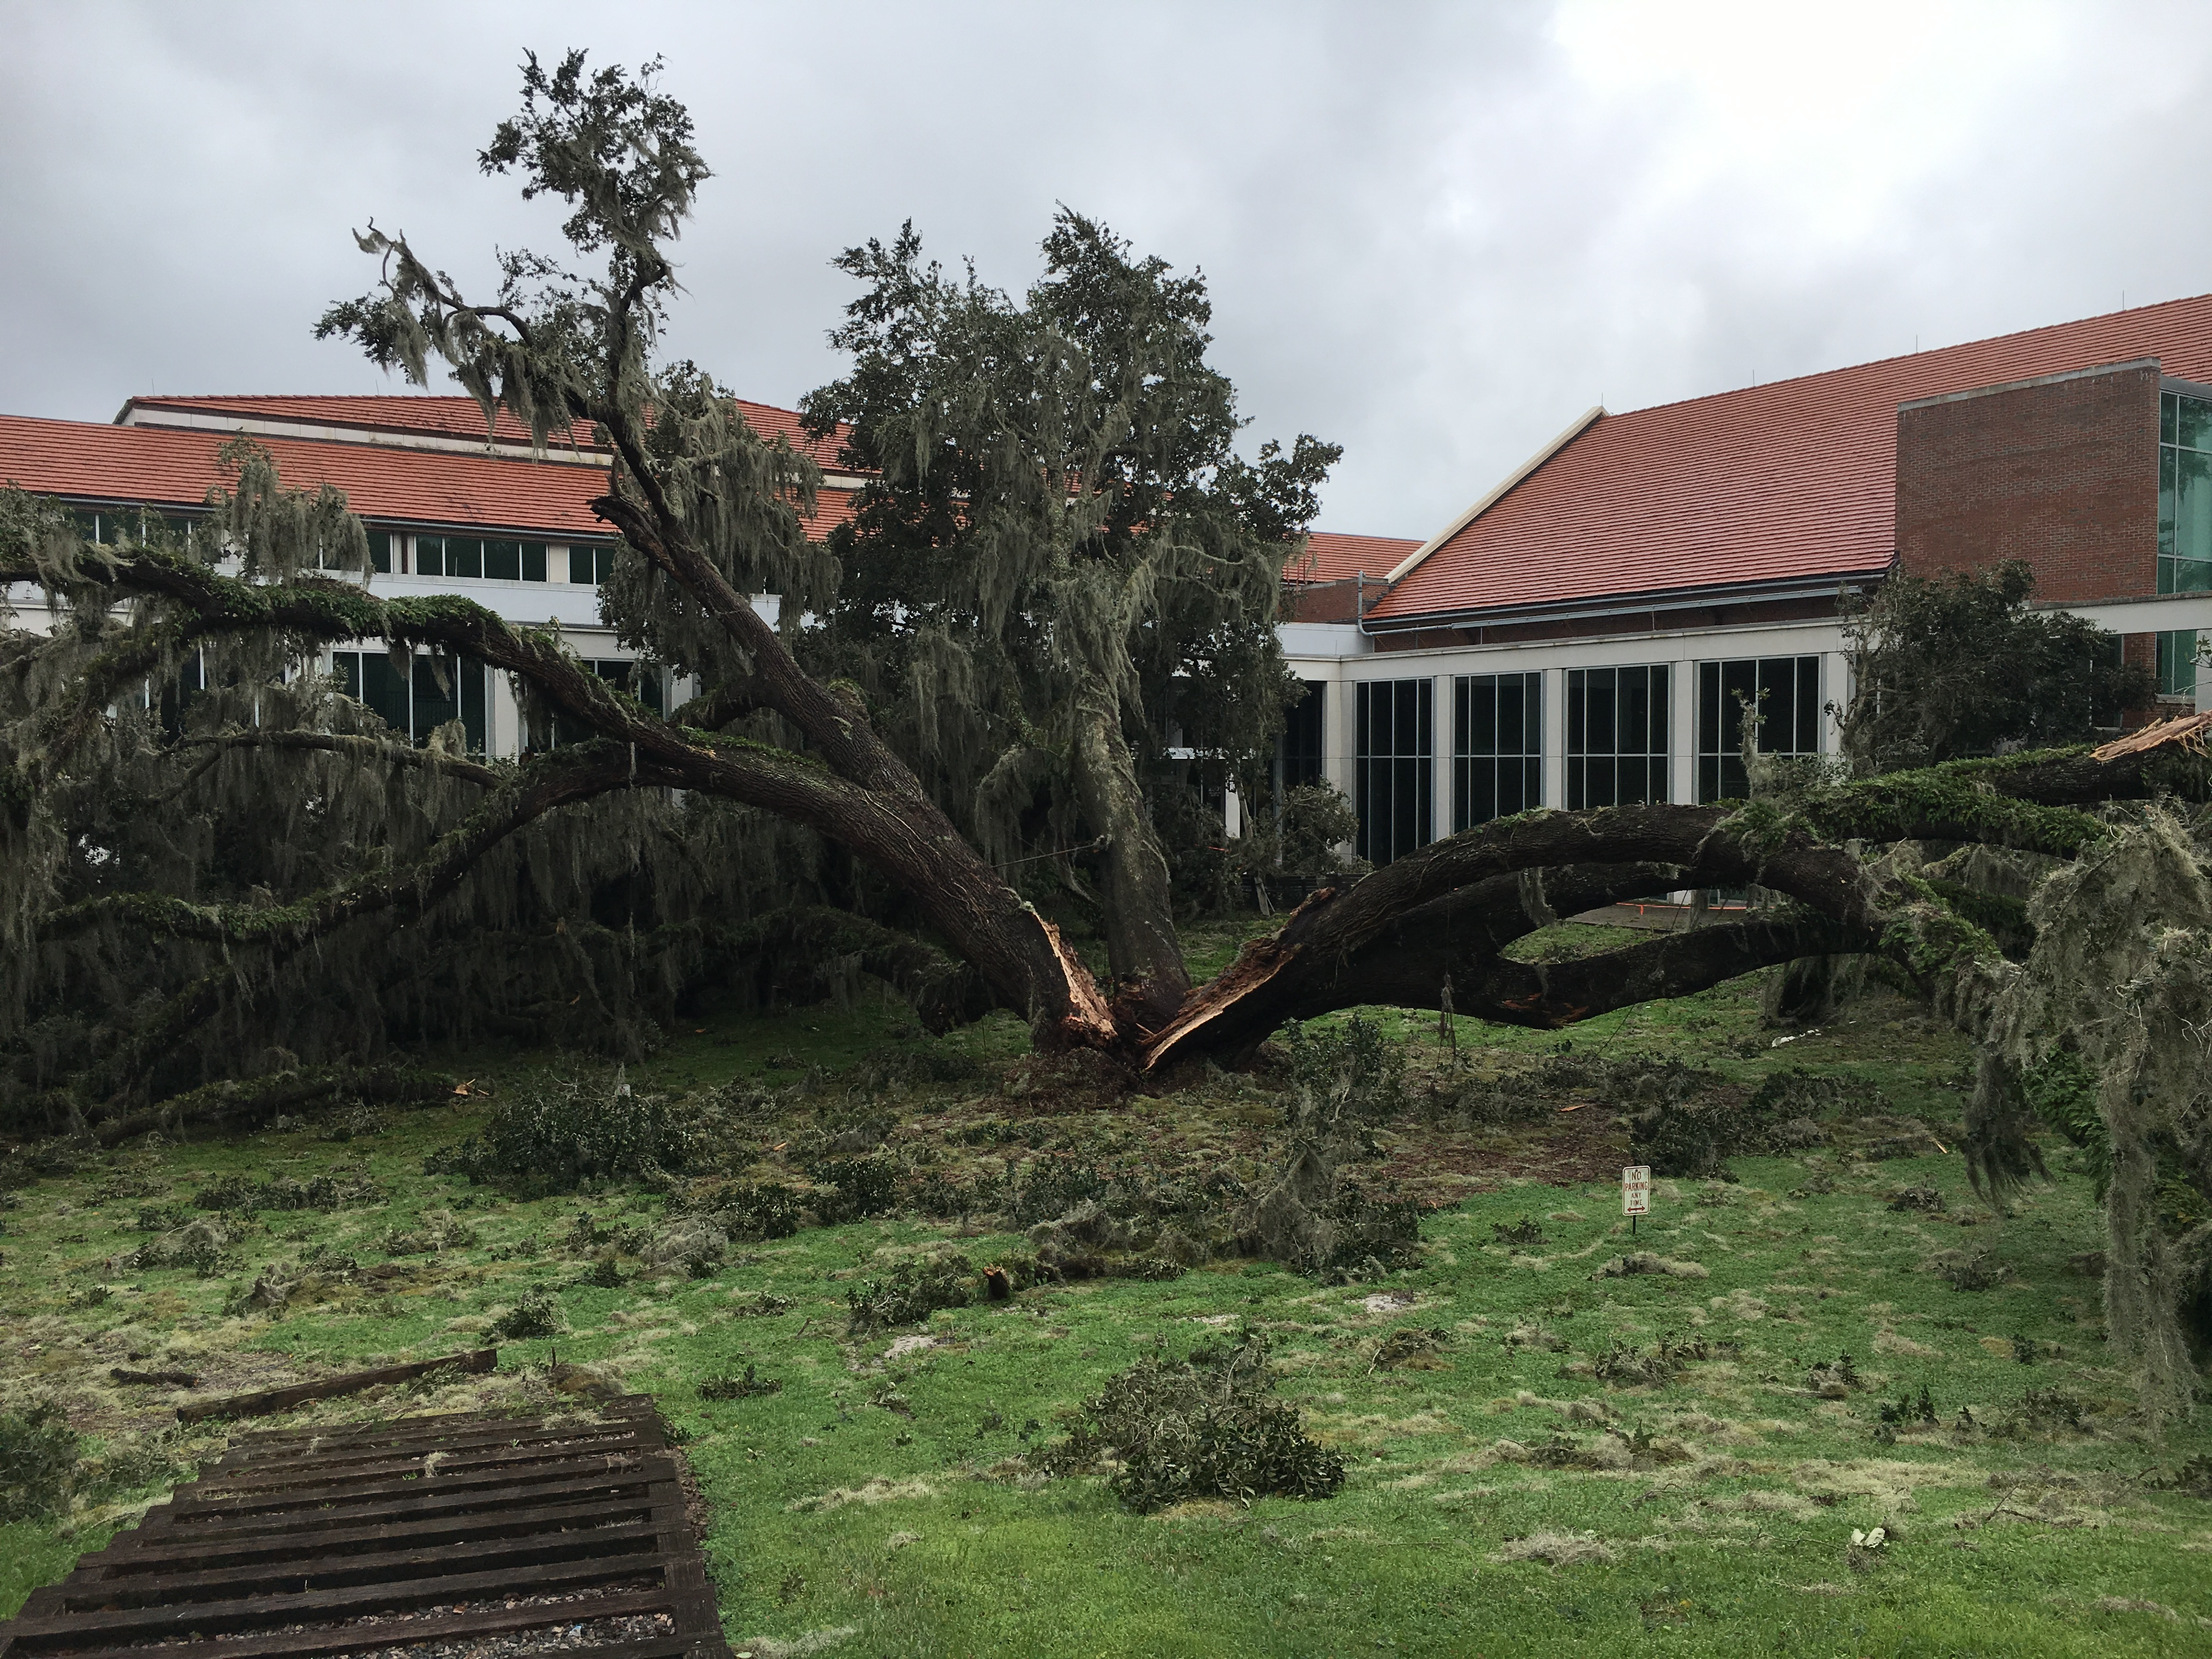
\includegraphics[height=5cm]{bigtree_down.JPG}
    \captionof{figure}
        [The Physics Tree before and after Hurricane Irma]
        {The Physics Tree in front of NPB.
        \;A) Before Hurricane Irma.
        \;B) After Hurricane Irma.
        }
\end{multiFigure}
%%%%%%%%%%%%%%%%%%%%